% !TeX root=../main.tex
\chapter{روش پیشنهادی}
%\thispagestyle{empty} 
\section{مقدمه} 
در این فصل، روش پیشنهادی مورد استفاده برای توسعه و ارزیابی سیستم گفتگوی وظیفه‌گرا با رویکرد شخصی‌سازی مورد بررسی قرار می‌گیرد. این روش شامل طراحی معماری سیستم با تمرکز بر حل چالش‌های اساسی نظیر مشکل شروع سرد، شخصی‌سازی مبتنی بر نماگر کاربر، بهره‌گیری از مدل‌های زبانی بزرگ، و تضمین حق فراموشی است. 
همچنین به مراحل پیش‌پردازش داده‌ها، استفاده از تکنیک‌های تنظیم سریع و استخراج موجودیت‌های کلیدی از ورودی کاربران پرداخته می‌شود. در نهایت، مکانیزم‌های جمع‌آوری بازخورد و ارزیابی عملکرد سیستم توضیح داده خواهند شد تا نقش آن‌ها در بهبود پویای سیستم مشخص شود.

نام روش پیشنهادی فوق MindMeld است. MindMeld در واقع ادغام هوشیارانه ذهن و ماشین برای گفتگوهای شخصی‌سازی‌شده است.


ادغام هوشیارانه در واقع بیانگر ترکیب دقیق و هدفمند داده‌ها و الگوریتم‌هاست. ذهن و ماشین نشان‌دهنده تعامل بین کاربر (ذهن) و سیستم هوش مصنوعی (ماشین) است که در قلب رویکرد فوق قرار دارد. همچنین گفتگوهای شخصی‌سازی‌شده به هدف اصلی که پاسخ های سفارشی‌شده و منطبق با نیازهای کاربر است.

\section{جمع آوری و آماده سازی داده ها}
\label{chap:dataset}
این بخش به فرآیند آماده‌سازی داده‌ها برای توسعه سیستم گفتگوی وظیفه‌گرا را توضیح می‌دهد. هدف این است که داده‌های خام از منابع مختلف، از جمله مجموعه‌داده 
مووی لنز%
\LTRfootnote{MovieLens}
، به داده‌های گفتگو‌محور تبدیل شوند که مناسب برای انجام تنظیم سریع یا یادگیری درون‌متنی%
\LTRfootnote{In-Context Learning}
 هستند.
\begin{enumerate}
\item
انتخاب و بررسی مجموعه‌داده مووی لنز\\
برای تحلیل اولیه و ایجاد مجموعه‌داده مکالمه‌محور، از 
\href{https://www.kaggle.com/datasets/garymk/movielens-25m-dataset}{مجموعه داده مووی لنز 25 میلیون}
 استفاده شده است. این مجموعه داده به طور گسترده در حوزه‌های مختلف از جمله سیستم‌های توصیه‌گر و فیلتر مشارکتی استفاده می‌شود. منبع این مجموعه داده سایت 
\href{https://www.kaggle.com}{کگل}
 است که حاوی بیش از 25 میلیون رتبه‌بندی، 1 میلیون برنامه برچسب و ابرداده برای 62000 فیلم است. همچنین این مجموعه داده بیش از 20 میلیون رتبه بندی فیلم و برچسب گذاری‌های کاربران است که از سال 1995 جمع آوری کرده است. \\


ویژگی‌های کلیدی این مجموعه داده به شرح زیر است.
\begin{itemize}
\item
امتیازات کاربران: داده‌های صریح شامل رتبه‌بندی کاربران برای فیلم‌ها (1 تا 5 ستاره).
\item
تگ‌ها: عبارات یا کلمات کلیدی مرتبط با فیلم که توسط کاربران اعمال می‌شوند.
\item
ژانرها: دسته‌بندی‌های فیلم، از جمله ژانرهای اکشن، کمدی، درام و غیره.
\item
اطلاعات زمانی: مهر زمانی مربوط به تعاملات کاربران با فیلم‌ها.
\end{itemize}

در این پژوهش، از دیتاست مووی لنز به عنوان یک مثال کاربردی استفاده شده است. همانطور که ذکر شد، این دیتاست شامل اطلاعات مربوط به علایق کاربران در حوزه فیلم‌ها و امتیازدهی به آن‌ها است. با این حال، روش پیشنهادی این پژوهش تنها محدود به این حوزه نیست و می‌تواند برای دیتاست‌های دیگر در حوزه‌های مختلف مانند موسیقی، کتاب، محصولات خرید آنلاین، یا حتی خدمات آموزشی تطبیق داده شود. این انعطاف‌پذیری به دلیل طراحی عمومی الگوریتم‌ها و عدم وابستگی به ویژگی‌های خاص دیتاست است.
 
جزییات روش پیشنهادی که به طور کامل در بخش%
\ref{sec:architecture}
 بیان خواهدشد شامل مراحلی است که مستقل از نوع داده‌ها عمل می‌کنند.

به عنوان مثال، در حوزه فیلم‌ها، داده‌های ورودی شامل امتیازهای کاربران به فیلم‌ها و ژانرهای مورد علاقه آن‌ها است. اما این ورودی‌ها می‌توانند به راحتی با داده‌های دیگری مانند امتیازهای کاربران به آهنگ‌ها یا کتاب‌ها جایگزین شوند. در ادامه، با استفاده از دیتاست مووی لنز، نحوه عملکرد این روش را در قالب یک مثال کاربردی شرح می‌دهیم." 

\item
ترکیب و یکپارچه‌سازی مجموعه‌داده
 
برای ایجاد یک مجموعه داده منسجم و مناسب سیستم گفتگو نیاز به داده‌هایی داریم که دارای ماهیت مکالمه‌محور باشند یا به بیان دیگر این داده‌ها باید به صورت جفت مقدارهای پرسه و پاسخ باشند تا بتوان مدل زبانی خود را با استفاده از این داده ها آموزش داد.

در وهله اول جهت ایجاد یک مجموعه داده متشکل از فیلم ها، نظرات و امتیازات کاربران و غیره به صورت یکجا، فایل‌های امتیازات کاربران، تگ‌های آنها که به فیلم‌های مختلف داده‌اند را بر اساس ستون‌های مشترک مانند آیدی فیلم و آیدی کاربران ادغام کرده و یک مجموعه داده شامل 126 هزار کورد ایجاد نمودیم.

خروجی نهایی این مجموعه داده شامل ستون های زیر است:
\begin{itemize}
\item
آیدی کاربر: شناسه یکتای هر کاربر.
\item
آیدی فیلم: شناسه یکتای هر فیلم.
\item
رتبه‌بندی: امتیاز داده‌شده توسط کاربر.
\item
تگ‌ها: برچسب‌های کاربران برای هر فیلم.
\item
ژانرها: دسته‌بندی‌های فیلم.
\end{itemize}

% جدول نمونه برای فیلدهای موجود در مجموعه داده movieRatingTag
\begin{table}[ht]
    \centering
    \caption{نمونه‌ای از داده‌های یکپارچه شده از مجموعه داده مووی لنز}
    \label{tab:movielens-sample}
    \renewcommand{\arraystretch}{1} % Adjust row height
    \begin{tabularx}{\textwidth}{|>
{\centering\arraybackslash}p{0.1\textwidth}|>
{\centering\arraybackslash}p{0.1\textwidth}|>
{\centering\arraybackslash}p{0.1\textwidth}|>
{\centering\arraybackslash}X|>
{\centering\arraybackslash}X|>
{\centering\arraybackslash}X|}
        \hline
        \textbf{userId} &
        \textbf{movieId} &
        \textbf{rating} &
        \textbf{title} &
        \textbf{genres} &  
        \textbf{tags} \\ 
        \hline
        1629 & 2 & 5.3 & Jumanji (1995) & Adventure, Fantasy & time travel \\ 
        \hline
    \end{tabularx}
\end{table}

\item
ایجاد مجموعه داده پیام‌های مکالمه‌محور:

برای آماده‌سازی مجموعه داده به فرم پرسش و پاسخ‌های گفتگو‌محور مراحل زیر انجام شد:
\begin{itemize}
\item
محاسبه شباهت کسینوسی:
\begin{itemize}
\item
تگ‌های فیلم‌ها به صورت ماتریس برداری با استفاده از CountVectorizer تبدیل شدند.
\item
شباهت کسینوسی بین بردارهای تگ محاسبه شد تا فیلم‌های مشابه شناسایی شوند.
\item
فیلم‌هایی با شباهت بالای 90٪ به عنوان موارد پیشنهادی برای همان فیلم در نظر گرفته شدند.
\end{itemize}

\item
فرمت‌دهی داده‌ها به صورت مکالمه‌ای:

از داده‌های شناسایی‌شده، ساختارهایی با پرسش و پاسخ ایجاد شد.\\
نمونه پرسش:
\begin{quote}
\begin{LTR}
Recommend movies similar to Harry Potter and the Philosopher's Stone
\end{LTR}
\end{quote}
نمونه پاسخ:
\begin{quote}
\begin{LTR}
"Harry Potter and the Chamber of Secrets" for its Hogwarts sequel, "The Lord of the Rings: The Fellowship of the Ring" for its fantasy adventure and "Percy Jackson The Olympians: The Lightning Thief" for its mythological adventure
\end{LTR}
\end{quote}
\end{itemize}

\item
محاسبه شباهت کسینوسی:
برای شناسایی شباهت بین فیلم‌ها و ایجاد جفت‌های پرسش و پاسخ مناسب، از شباهت کسینوسی استفاده شد. رابطه شباهت کسینوسی برای دو بردار متنی A و B به صورت رابطه ی %
\ref{eq:cosineSimilarity}
 تعریف می‌شود:

 
\begin{equation}
\label{eq:cosineSimilarity}
\text{شباهت کسینوسی} = \frac{\sum_{i=1}^{n} A_i \cdot B_i}{\sqrt{\sum_{i=1}^{n} A_i^2} \cdot \sqrt{\sum_{i=1}^{n} B_i^2}}
\end{equation}


که در آن مقادیر Ai​ و Bi​ مقدار ویژگی i در بردارهای A و B هستند. همچنین مقدار n برابر با تعداد ویژگی‌ها (کلمات کلیدی یا تگ‌های فیلم‌ها در اینجا) هستند.

این رابطه تضمین می‌کند که شباهت بین دو بردار بر اساس جهت آن‌ها و نه اندازه‌شان محاسبه شود. شباهت کسینوسی معمولاً برای داده‌های متنی و برداری در تحلیل‌های پردازش زبان طبیعی و مدل‌های توصیه‌گر به کار می‌رود.

روش پیاده‌سازی این رابطه به صورت فوق است:
\begin{itemize}
\item
تبدیل تگ‌ها به بردارها: با استفاده از تکنیک CountVectorizer، تگ‌های متنی مربوط به فیلم‌ها به بردارهای عددی تبدیل شدند. این تکنیک بسته کلمات%
\LTRfootnote{Bag of Words (BoW)}
 برای نماگر‌سازی متنی استفاده می‌شود.
\item
محاسبه شباهت: شباهت کسینوسی بین بردارهای مربوط به فیلم‌ها محاسبه شد. همانطور که بیان شد، فیلم‌هایی که شباهت آن‌ها بیش از 90٪ بود، به عنوان فیلم‌های مشابه در نظر گرفته شدند.
\end{itemize}

جهانگیر و همکاران%
\cite{singh2020movie}
 با استفاده از تکنیک فوق، الگوریتم‌هایی توسعه داده شده‌اند که از داده‌های مشابه مووی لنز برای شناسایی فیلم‌های مشابه استفاده می‌کنند. برای مثال، با بهینه‌سازی عبارات کلیدی و اضافه کردن وزن به ژانرها، دقت مدل‌ها افزایش یافته است.


\item
گسترش تنوع پرسش و پاسخ:

با استفاده از فیلم مرجع و فیلم هایی که شباهت کسینوسی بالایی نسبت به فیلم فوق داشته اند، مجموعه ای از فیلم ها به همراه فیلم های مشابه با آن ها را در دسترس خواهیم داشت که می تواند در ادامه ایجاد مجموعه داده مکالمه‌محور کمک کند.\\
برای شباهت بیشتر داده‌ها به گفتگوهای روزمره، 50 قالب مختلف برای پرسش و 50 قالب برای پاسخ طراحی شد.


به عنوان مثال فیلم Hard Die را در نظر بگیرید، یک نمونه پرسه به فرم زیرخواهد بود:
\begin{quote}
\begin{LTR}
Looking for hidden gems like 'Die Hard 1988' in the action genre
\end{LTR}
\end{quote}

برای فیلم های با ژانرهای مختلف یکی از ژانرها به تصادف برای ایجاد مجموعه داده استفاده می‌شود.
همچنین یک نمونه پاسخ کاندید به صورت زیر خواهد بود:
\begin{quote}
\begin{LTR}
Finding more action films similar to ‘Die Hard 1988'. How about: Hellboy 2004
\end{LTR}
\end{quote}


\item
ایجاد مجموعه‌داده نهایی: 

ساختار مجموعه‌داده نهایی به سبک زیرخواهد بود
\begin{itemize}
\item
ورودی: شامل سوالات کاربران در قالب طبیعی
\item
خروجی: لیست فیلم‌های پیشنهادی
\item
نام فیلم: فیلم ذکر‌شده در سوال
\item
سال: سال انتشار فیلم
\item
ژانر: ژانرهای فیلم.

\end{itemize}

با این روش، مجموعه‌داده‌ای شامل 210 هزار ردیف مکالمه‌ای ایجاد شد که برای مراحل بعدی در توسعه سیستم گفتگوی وظیفه‌گرا مورد استفاده قرار گرفت.


\end{enumerate}

\section{معماری سیستم}
\label{sec:architecture}
\subsection{مراحل تولید پاسخ}

این معماری برای تقویت تعامل کاربر با سیستم گفتگو وظیفه‌گرا و با  توجه به چالش‌های کلیدی مانند مسائل شروع سرد، شخصی‌سازی، استفاده از مدل های بازی تنظیم شده و رعایت حق فراموشی طراحی شده‌است. هر ماژول و اجزای آن برای بهبود سازگاری سیستم، رضایت کاربر و عملکرد خاص دامنه مورد نظر طراحی شده‌اند. در ادامه کلیّت معماری پیاده‌سازی‌شده توضیح داده‌شده و در بخش‌های آتی، هر قسمت به صورت مجزا و مفصل تر مورد بحث قرار خواهد گرفت.

جهت سهولت درک توضیحات شکل%
\ref{fig:architecture}
شماره گذاری در قسمت های مختلف آن انجام شده است که در هنگام توضیح هر قسمت، شماره آن نیز رو به روی آن آورده شده است.


\begin{figure}[ht]
	\centerline{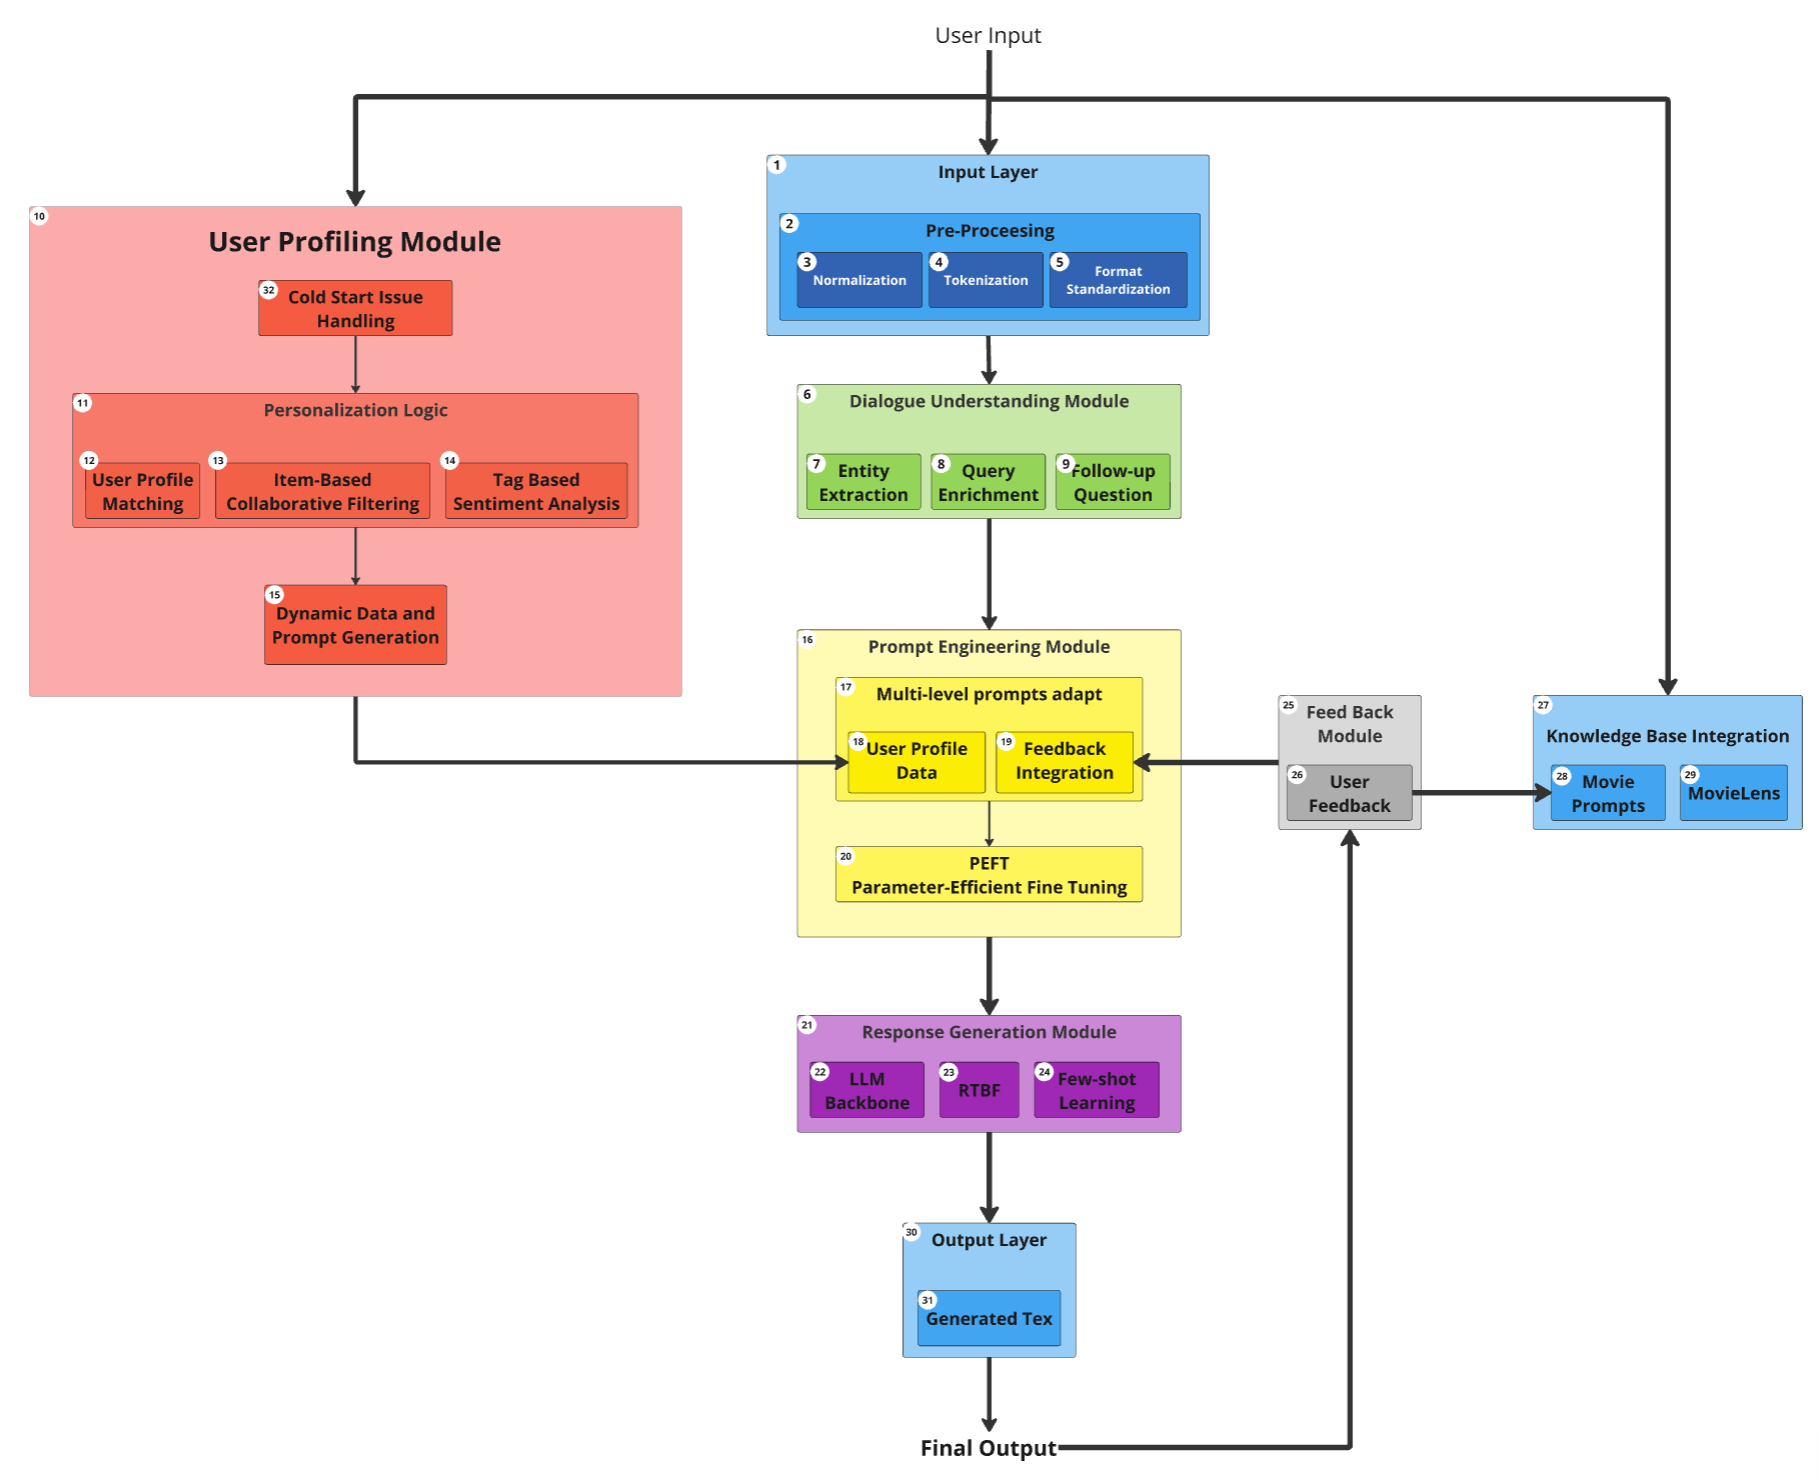
\includegraphics[width=1.0\textwidth]{architecture}}
	\caption{معماری سیستم}
	\label{fig:architecture}
\end{figure}


\begin{enumerate}
\item
 لایه ورودی
\begin{itemize}
\item
ورودی کاربر(بخش 1): این ماژول نقطه شروع دسترسی کاربر جهت پرسش سوال خود است. در این سیستم گفتگو، پرسه های مبتنی بر متن از کاربر پذیرفته می‌شود.
\item
پیش پردازش (بخش 2):
در مرحله پیش‌پردازش، داده‌های خام تمیز شده و ویژگی‌های ناقص یا نویزی حذف می‌شوند. اولین مرحله از پیش‌پردازش پرسه کاربر، 
عادی سازی%
\LTRfootnote{Normalization}
  (بخش 3) است. در این مرحله سیستم قالب متن ورودی به عنوان مثال، حروف کوچک و علامت‌گذاری را استاندارد می کند.
\item
توکن‌بندی کردن%
\LTRfootnote{Tokenization}
 (بخش 4) :متن به واحدهای قابل مدیریت (کلمات یا عبارات) شکسته می‌شود.
\item
استاندارد‌سازی فرمت%
\LTRfootnote{format standardization}
 (بخش 5) که سازگاری با ماژول‌های پردازش مراحل بعدی را تضمین می‌کند.
\end{itemize}

فرآیندهای مرحله پیش‌پردازش به طور کلی مستقل از حوزه کاربرد است و می‌تواند برای هر نوع داده‌ای اعمال شود. به عنوان مثال، در دیتاست مووی لنز، این شامل حذف رکوردهای ناقص امتیازدهی کاربران به فیلم‌ها می‌شود. اما در یک دیتاست مربوط به خرید آنلاین، این مرحله می‌تواند شامل حذف محصولاتی باشد که توضیحات ناقص دارند.
\item
 ماژول درک گفتگو (بخش 6)
\begin{itemize}
\item
استخراج موجودیت%
\LTRfootnote{Entity Extraction}
 (بخش 7) : موجودیت‌های کلیدی مانند نام فیلم و ژانرها را در پرسه کاربر را شناسایی می‌کند. اما این رویکرد به هیچ وجه محدود به فیلم‌ها نیست و می‌تواند برای استخراج ویژگی‌های دیگری مانند قیمت، برند، یا رنگ محصولات در دیتاست‌های خرید آنلاین استفاده شود.
\item
تولید‌کننده سوال بعدی%
\LTRfootnote{Follow-up question}
 (بخش 9) : برای روشن‌کردن ورودی‌های مبهم یا ناقص کاربر، درخواست‌های بعدی ایجاد می کند.
\item
غنی‌سازی پرس‌وجو%
\LTRfootnote{Query Enrichment}
 (بخش 8) : داده‌های ورودی را به صورت پویا تنظیم و اصلاح می‌کند تا درک و زمینه سیستم را بهبود بخشد. به عنوان مثال به مدل زبانی پرسه کامل به همراه فراداده هایی چون ژانر موردنظر کاربر و فیلم مورد بحث را به همراه پرسه اصلی کاربر به ورودی مدل جهت انجام عملیات تنظیم سریع بعدی ارسال می‌کند.
\end{itemize}

\item
 ماژول نماگر کاربری (بخش 10)
\begin{itemize}
\item
رسیدگی به مشکل شروع سرد (بخش 32):\\
 زمانی که حداقل داده های کاربر در دسترس نباشد، ماژول از یک تا پنج ژانرهای مورد علاقه کاربر را از وی دریافت می‌کند و علاوه بر آن با به کارگیری فیلترمشارکتی مبتنی بر آیتم،  ترجیحات کاربر را استنتاج و استفاده می‌کند.
\item
منطق شخصی سازی (بخش 11):
\begin{itemize}
\item
تطابق نماگر کاربر (بخش 12): از داده‌های موجود کاربر، مانند امتیازات وی، تگ ها یا ژانرهای مورد علاقه (مانند استفاده از مجموعه داده مووی‌لنز) استفاده می‌کند.
\item
تحلیل احساسات مبتنی بر برچسب (بخش 14): لحن و اولویت درخواست کاربر را بر اساس داده های برچسب‌گذاری‌شده تجزیه‌وتحلیل می‌کند و آیتم‌هایی که وی به آنها تگ‌هایی با لحن مثبت و خوب داده است را استخراج می‌کند.
\item
استفاده از فیلتر مشارکتی مبتنی‌بر آیتم جهت استخراج ژانرها و فیلم‌هایی که کاربر احتمالا به آنها علاقه دارند (بخش 13).
\end{itemize}

\item
تولید داده‌های پویا و تولید پرامپت (بخش 15): رفتار سیستم را در زمان واقعی با استفاده از داده‌های نماگر کاربر تطبیق و شخصی می‌کند و یک پرسه شخصی‌سازی‌شده را به مدل ارسال می‌کند.
\end{itemize}


\item
ماژول مهندسی پرامپت (بخش 16)
\begin{itemize}
\item
تنظیم سریع: 
تنظیم دقیق پارامترهای کارآمد%
\LTRfootnote{Parameter Efficient Fine Tuning(PEFT)}
 (بخش 20) برای کاهش منابع مورد نیاز و در عین حال تنظیم مدل‌های پایه برای ویژگی خاص دامنه پیاده‌سازی در این قسمت اجرایی می‌شوند. این قسمت پیام‌های چند سطحی را ایجاد می‌کند که به صورت پویا بر اساس نماگر‌ها و تنظیمات کاربر تطبیق می‌یابد.
\item
یکپارچه سازی بازخورد (بخش 19):
رتبه‌بندی کاربران (پسندیدن/نپسندیدن/خنثی) را در پاسخ‌های سیستم جمع‌آوری می‌کند و به طور مکرر درخواست‌ها را به روز می‌کند تا بهتر با انتظارات کاربر هماهنگ شود.
\end{itemize}

\item
ماژول تولید پاسخ (بخش 21)
\begin{itemize}
\item
استفاده از مدل زبانی (بخش 22):\\
با یک مدل زبانی که با دستورات مخصوص دامنه تنظیم شده‌است تا پاسخ‌های مرتبط و منسجمی ایجاد کند.
\item
حق فراموشی (بخش 23):\\
با ناشناس‌کردن ورودی‌های کاربر و حذف داده‌هایی که مدل با استفاده از آنها برای یک کاربر خاص شخصی‌سازی شده است در صورت درخواست، حریم خصوصی کاربر را تضمین می‌کند.
\item
آموزش چند شات (بخش 24):\\
به سرعت با ورودی‌های جدید با استفاده از نمونه‌های چند شات بدون نیاز به بازآموزی گسترده سازگار می‌شود و از پاسخگویی به سناریوهای جدید اطمینان می‌دهد.
\end{itemize}

\item
جمع آوری و ارزیابی بازخورد 
\begin{itemize}
\item
بازخورد کاربر (بخش 26): بازخورد کاربر (پسندیدن/نپسندیدن/خنثی) برای هر یک از پاسخ های سیستم را از کاربران جمع آوری می‌کند.
\item
تنظیم تکراری%
\LTRfootnote{Iterative Tuning}
: به طور مداوم عملکرد سیستم را بر اساس بازخورد جمع آوری شده کاربران اصلاح می کند.
\end{itemize}


\item
لایه خروجی (بخش 30)

خروجی های متن تولید شده، پاسخ های ساختارمند و مبتنی بر متن را ارائه می دهد که برای سیستم گفتگو مبتنی بر چت بهبود یافته اند.

\end{enumerate}

\subsection{ویژگی های کلیدی پرداخته شده در معماری}
در معماری ارائه شده در شکل%
\ref{fig:architecture}
 ،به مشکلات زیر پرداخته است.
 
\begin{enumerate}
\item
مشکل شروع سرد:
از طریق فیلتر مشارکتی مبتنی بر آیتم و تنظیم دقیق مدل با استفاده از تنظیمات پیش‌فرض و ترجیحات دریافت شده انجام می‌شود.
\item
حق فراموشی:
حق فراموشی یکی از اصول مهم حفظ حریم خصوصی کاربران است. این حق به کاربران اجازه می‌دهد تا درخواست حذف اطلاعات شخصی خود را از پلتفرم‌ها ارائه دهند. این شامل اطلاعات حساس مانند علایق، سابقه جستجو، یا حتی کل حساب کاربری است.

سازگاری با ورودی های جدید:
سیستم از تکنیک‌های پیشرفته‌ای مانند یادگیری چند شات استفاده می‌کند تا بتواند به راحتی با سناریوهای جدید سازگار شود. این تکنیک به سیستم اجازه می‌دهد تا با مشاهده تنها چند نمونه جدید، به سرعت عملکرد خود را بهبود بخشد. علاوه بر این، تنظیم سریع مجدد نیز به کار گرفته می‌شود. این فرآیند شامل به‌روزرسانی مدل بدون نیاز به آموزش مجدد کامل است. به این ترتیب، سیستم می‌تواند به سرعت به تغییرات محیطی یا نیازهای جدید کاربران پاسخ دهد و کارایی خود را حفظ کند.

این رویکردها، سیستم را انعطاف‌پذیرتر و کاربرپسندتر می‌کنند.
\end{enumerate}


\section{ماژول درک مکالمه}
ماژول درک مکالمه%
\LTRfootnote{Dialogue Understanding Module}
 (بخش 6) به نحوه پردازش پرسش‌های کاربر برای آماده‌سازی داده‌های ورودی مناسب جهت استفاده در مدل می پردازد. این ماژول به‌عنوان نقطه شروع تعاملات کاربر با سیستم عمل کرده و با تجزیه و تحلیل ورودی‌های کاربر (پرامپت‌ها) و اضافه کردن جزئیات مفقود، پرسش‌های کامل و ساختاریافته‌ای را برای مدل تولید می‌کند.

فرآیند درک مکالمه از سه گام اصلی تشکلیل شده است که به شرح زیر است.
\begin{enumerate}
\item

استخراج موجودیت‌های نام‌گذاری‌شده%
\LTRfootnote{Named Entity Recognition (NER)}
 (بخش 7) برای درک بهتر درخواست‌های کاربر، از تکنیک‌های استخراج موجودیت‌های نام‌گذاری‌شده استفاده می‌شود.\\
شناسایی موجودیت نام‌گذاری شده یک کار اساسی در پردازش زبان طبیعی است که شامل شناسایی و دسته‌بندی موجودیت‌های نام‌گذاری شده در یک سند متنی به دسته‌های از پیش تعیین‌شده است
\cite{singh2020movie}
.
این دسته ها معمولاً عبارتند از:
\begin{itemize}
\item
شخص: نام افراد، مانند «جان اسمیت»
\item
سازمان: نام شرکت‌ها، مؤسسات یا سازمان‌ها، مانند "Google"
\item
منطقه: نام مکان‌های جغرافیایی، مانند «نیویورک»
\item
تاریخ: تاریخ‌ها، زمان‌ها یا دوره‌ها، مانند "01-01-2022"
\item
رویداد: نام رویدادها، مانند «جام جهانی»
\end{itemize}

هدف استخراج موجودیت‌های نام‌گذاری‌شده، شناسایی و طبقه‌بندی خودکار این موجودیت‌های نام‌گذاری شده در یک متن است که می‌تواند برای برنامه‌های مختلف استفاده شود، مانند:
\begin{itemize}
\item
استخراج اطلاعات: استخراج اطلاعات مرتبط از داده‌های متنی
\item
خلاصه‌سازی متن: خلاصه‌کردن متن براساس موجودیت‌های شناسایی‌شده
\item
تجزیه‌وتحلیل احساسات: تجزیه‌وتحلیل احساس متن براساس موجودیت‌های ذکرشده
\item
پاسخ به سؤال: پاسخ به سؤالات براساس نهادهای شناسایی‌شده
\end{itemize}


چندین رویکرد برای استخراج موجودیت‌های نام‌گذاری‌شده وجود دارد %
\cite{corecco2024evolution}

، از جمله:
\begin{itemize}
\item
رویکرد مبتنی بر قانون: استفاده از قوانین از پیش تعیین‌شده برای شناسایی موجودیتها
\item
رویکرد نظارت شده: با استفاده از الگوریتم‌های یادگیری ماشین آموزش‌داده‌شده بر روی داده‌های برچسب‌دار
\item
رویکرد بدون نظارت: استفاده از خوشه‌بندی یا تکنیک‌های دیگر برای شناسایی موجودیت‌ها بدون داده‌های برچسب‌دار
\item
رویکرد یادگیری عمیق: استفاده از شبکه‌های عصبی برای یادگیری الگوهای موجود در داده‌ها%
\cite{fan2024recommender}

\end{itemize}


هدف اصلی در این بخش از سیستم شناسایی موارد زیر است:
\begin{itemize}
\item
نام فیلم: برای یافتن نام فیلم در متن پرامپت، از روش‌های ساده‌ای مانند استفاده از نقل‌قول‌ها استفاده می‌شود. اگر نام فیلم داخل نقل‌قول باشد، سیستم به‌طور مستقیم آن را به‌عنوان یک فیلم شناسایی می‌کند و از سایر روش‌های پردازش صرف نظر می‌کند. در غیر این صورت با استفاده از پردازش زبانی طبیعی تلاش می‌کند که نام فیلم را از عبارت وارد شده استخراج کند.
\item
ژانر فیلم: سیستم تلاش می‌کند تا ژانر را از میان لیستی از ژانرهای از پیش تعریف‌شده تشخیص دهد. ژانرهای موجود به شرح زیر است:
کمدی، موزیکال، هیجان‌انگیز، عاشقانه، مستند، ترسناک، جنایی، انیمیشن، فانتزی، ماجراجویی، علمی تخیلی، معمایی، کودکان، درام، جنگی، اکشن و وسترن.
\end{itemize}

استفاده از این تکنیک‌ها به سیستم کمک می‌کند تا اطلاعات اصلی از پرامپت استخراج شده و با دقت بیشتری پرسش کاربر پردازش شود. با این حال، برای حفظ سادگی، تمرکز ما در این بخش بر پاسخ‌های اولیه و پرسش‌های پیگیری است و سیستم از مدل‌های پیچیده‌تر استخراج موجودیت‌های نام‌گذاری‌شده صرف نظر کرده است.

\item
پرسش‌های پیگیری (بخش 9):

اگر کاربر اطلاعاتی ناقص ارائه دهد (مانند عدم ذکر فیلم یا ژانر)، سیستم به صورت خودکار پرسش‌های پیگیری تولید می‌کند. این پرسش‌ها با استفاده از الگوهای از پیش تعریف‌شده طراحی شده‌اند. برای مثال:
\begin{itemize}
\item
اگر نه نام فیلم و نه ژانر در پرسه کاربر نباشد، «لطفا نام فیلم و ژانر مورد نظر خود را ذکر کنید»
\item
اگر نام فیلم مشخص نباشد: «لطفاً نام فیلم موردنظر خود را مشخص کنید؟»
\item
اگر ژانر ذکر نشده باشد: «آیا ژانر خاصی را مدنظر دارید؟»
\end{itemize}
کاربر می‌تواند به این پرسش‌ها پاسخ دهد و سیستم پاسخ‌های کاربر را به پرامپت اولیه اضافه می‌کند تا یک پرامپت کامل و ساختاریافته ایجاد شود.
\newline
هرچه یک پرسه جزییات دقیق‌تر مانند جزییات ژانر و نام فیلم را دارا باشد مدل توانایی تولید عبارات بهتر و متناسب تر برای کاربر خواهد بود که در نهایت به بهبود تجربه کاربری منجر خواهد شد.
\newline
برای حفظ انعطاف‌پذیری، کاربران می‌توانند از این مرحله عبور کرده و پرامپت اولیه خود را بدون تغییر ارسال کنند. این قابلیت، تجربه کاربری را بهبود  داده و امکان استفاده از سیستم را برای کاربران حرفه‌ای‌تر که می‌خواهند پرسش‌های خود را مستقیماً به مدل ارسال کنند، فراهم می‌کند.

\item

پیش‌پردازش پرامپت:

پیش‌پردازش پرامپت از طریق ماژول درک مکالمه، تضمین می‌کند که مدل داده‌های ورودی کامل و دقیق دریافت می‌کند. همچنین احتمال بروز خطا یا پاسخ‌های نامرتبط کاهش می‌یابد و  تعاملات کاربر به شکلی ساختاریافته‌تر و قابل‌فهم‌تر برای مدل تبدیل می‌شود.

به عنوان مثال، اگر کاربر پرامپت زیر را وارد کند: 
\begin{displayquote}
\begin{LTR}
"I need movies similar to Inception"
\end{LTR}
\end{displayquote}

سیستم از استخراج موجودیت‌های نام‌گذاری‌شده برای استخراج نام فیلم ("Inception") استفاده می‌کند.
اگر ژانری مشخص نشده باشد، سیستم پرسشی مانند: «آیا ژانر خاصی را برای پیشنهاد مدنظر دارید؟» ارائه می‌دهد.
پاسخ کاربر به این پرسش‌ها اضافه شده و پرامپت نهایی، به شکل: 

\begin{displayquote}
\begin{LTR}
"I need movies similar to Inception in the Sci-Fi genre"
\end{LTR}
\end{displayquote}
به مدل ارسال می‌شود.
\\
این مرحله از پیش‌پردازش پرامپت، تضمین می‌کند که تعاملات کاربر با سیستم گفتگوی وظیفه‌گرا در فازهای بعدی (تولید پاسخ) بهینه باشد. علاوه بر این، رویکرد ساده و مؤثر آن به حفظ کارایی و پاسخگویی سریع سیستم کمک می‌کند.

خروجی نهایی این بخش ، عبارت ورودی کاربر به صورت کامل و همچنین نام فیلم و ژانر در صورت استخراج به صورت فراداده به عنوان ورودی به مدل وارد شده و عملیات های بعدی بر روی این عبارت صورت خواهد گرفت.

یک نمونه پرامپت جهت استفاده از مدل به صورت زیر خواهد بود
\begin{displayquote}
\begin{LTR}
{I need movies similar to Inception in the Sci-Fi genre} (metadatas: movie={Inception} - genre={Sci-Fi})
\end{LTR}
\end{displayquote}


\section{ماژول تولید پاسخ}
بخش تولید پاسخ%
\LTRfootnote{Response Generation}
 (بخش 21) به توضیح فرآیند تولید پاسخ‌های شخصی‌سازی‌شده و متناسب با زمینه برای سیستم گفتگوی پیشنهادی می‌پردازد. هدف از این بخش آن است که مدل با استفاده از داده‌هایی که در مرحله قبل و مختص هر کاربر تولید شده‌اند، تنظیم سریع شود. این داده‌ها شامل اطلاعاتی است که از پایگاه داده‌های فیلترشده استخراج شده و ترجیحات کاربر، مانند ژانرهای منتخب، را در خود جای داده است. علاوه بر این، مدل با پرامپت‌های خاصی که مبتنی بر ورودی‌های کاربر و دارای فراداده‌هایی مانند نام فیلم‌ها و ژانرهای آنها هستند، تنظیم می‌شود. این فرآیند به مدل اجازه می‌دهد تا پاسخ‌هایی دقیق، منطقی و سازگار با نیازهای کاربر تولید کند. 


این رویکرد نه تنها به تولید پاسخ‌های شخصی‌سازی‌شده کمک می‌کند، بلکه باعث می‌شود که سیستم بتواند به طور دقیق‌تری با ترجیحات و رفتارهای کاربران سازگار شود . از طرفی، استفاده از مدل زبانی بزرگ و تنظیم سریع، امکان تطبیق سریع با سناریوهای جدید را فراهم می‌کند . این ترکیب از داده‌های شخصی‌سازی‌شده و مدل‌های زبانی پیشرفته، به سیستم کمک می‌کند تا پاسخ‌هایی با کیفیت بالا و مرتبط با زمینه تولید کند.


مراحل اصلی در تولید پاسخ به شرح زیر است.
\begin{itemize}
\item
رمزگذاری پرسش کاربر: برای تبدیل پرسش‌های متنی به قالبی که مدل قادر به درک آن باشد، از توکنایزر استفاده می‌شود. این مرحله، پرسش‌های کاربر را به توالی‌های عددی تبدیل می‌کند.
\item
تولید پاسخ: از مدل زبانی تنظیم‌شده برای تولید پاسخ استفاده می‌شود. این مدل قادر است بر اساس ورودی‌ها، پاسخ‌هایی سازگار با تاریخچه تعاملات کاربر تولید کند.
\item
استخراج اطلاعات کلیدی: پس از تولید پاسخ، اطلاعاتی مانند نام فیلم‌ها یا ژانرها از پاسخ‌های تولیدشده استخراج می‌شوند. این اطلاعات برای ذخیره‌سازی و تحلیل‌های بعدی ثبت می‌گردند.
\end{itemize}


طراحی پارامترهای تولید پاسخ
\
برای اطمینان از کیفیت و تنوع پاسخ‌ها، پارامترهایی مانند doSample، top-k، و temperature تنظیم شده‌اند.
\begin{itemize}
\item
پارامتر doSample: این پارامتر برای ایجاد تنوع در پاسخ‌ها فعال شده‌ است. مقداردهی به این پارامتر به مدل امکان می‌دهد که پاسخ‌هایی غیرتکراری تولید کند.
\item
پارامتر top-k : این مقدار برای محدود‌کردن تعداد گزینه‌های کاندیدای تولید در هر مرحله به 100 تنظیم شده‌است.
\item
پارامتر temperature: این پارامتر بر نحوه‌ی تعادل میان تنوع و انسجام پاسخ‌ها تاثیر می‌گذارد و مقدار آن 
\num{0.8}
 تنظیم شده است.
\end{itemize}


\subsection{مدیریت تاریخچه تعاملات}

یکی از ویژگی‌های کلیدی سیستم این است که برای هر سوال جدید کاربر، تاریخچه گفتگو در نظر گرفته می‌شود. این تاریخچه تنها برای تعامل جاری کاربر استفاده می‌شود و از مکالمات چندمرحله‌ای برای تولید پاسخ پشتیبانی نمی‌شود. این رویکرد تضمین می‌کند که پاسخ‌ها مرتبط با موضوع باشند و پیچیدگی‌های اضافی را کاهش می‌دهد.


\subsection{فرآیند پاکسازی داده}

سیستم شامل مکانیزمی برای اجرای «حق فراموشی» است. این امکان به کاربر اجازه می‌دهد که درخواست حذف داده‌های پیشین خود را ارائه دهد. عملکرد پاک‌سازی داده‌ها به صورت زیر است:
\begin{itemize}
\item
بررسی ورودی کاربر برای تشخیص عبارت "RTBF"
\item
پاکسازی داده‌های ذخیره‌شده مرتبط با کاربر.
\item
بازگرداندن اطلاعات در مورد تعداد رکوردهای حذف‌شده.
\item
استفاده از بقیه داده ها جهت تنظیم سریع مجدد مدل و پاسخ به سوالات بعدی کاربر
\end{itemize}




\subsection{واکنش‌های کاربر به پاسخ‌ها}

\begin{itemize}
\item
سیستم بازخورد: پس از تولید هر پاسخ، کاربر می‌تواند واکنش خود که شامل «پسندیدم» یا «نپسندیدم» است را به پاسخ ثبت کند. در صورت عدم ارائه بازخورد، واکنش به صورت پیش‌فرض روی «هیچ» تنظیم می‌شود.
\item
هدف بازخورد: این مکانیزم به بهبود دقت و شخصی‌سازی پاسخ‌ها کمک می‌کند و امکان تحلیل بیشتر برای ارتقای مدل را فراهم می‌سازد. همچنین جهت دست یافتن به میزان کیفیت پاسخ های تولیدشده باید از بازخوردهای کاربران استفاده کرد که به تفضیل در بخش% 
\ref{chap:results}
 به آن پرداخته خواهد شد.


این بخش از سیستم، با بهره‌گیری از قابلیت‌های مدل‌های زبانی و تنظیم داده‌ها، تضمین می‌کند که پاسخ‌های تولیدشده متناسب با ورودی‌های کاربران و نیازهای آن‌ها باشند. علاوه بر این، طراحی انعطاف‌پذیر سیستم امکان ارتقا و بهبود آن در آینده را فراهم می‌کند.
\end{itemize}

\section{منطق شخصی سازی}
 
شخصی‌سازی یکی از اجزای کلیدی در سیستم‌های گفتگوی وظیفه‌گرا است که بر اساس ترجیحات و بازخورد کاربران، پاسخ‌هایی دقیق و مرتبط تولید می‌کند.این منطق بر اساس تحلیل داده‌های کاربران و به‌روزرسانی‌های پویا در مدل‌های تنظیم‌شده برای هر کاربر طراحی شده است.

این بخش به بررسی مراحل ایجاد مجموعه داده‌های شخصی‌سازی‌شده، مکانیزم بازخورد کاربر، و تأثیر این بازخورد در تولید پاسخ‌ها می‌پردازد.

ایجاد مجموعه داده‌های شخصی‌سازی‌شده%
\LTRfootnote{Personalized User Datasets}
، سنگ بنای سیستم‌های مبتنی بر شخصی‌سازی است که نیازهای کاربران را در مرکز توجه قرار می‌دهد. \\
یکی از گام‌های کلیدی در سیستم‌های توصیه‌گر و شخصی‌سازی گفتگوها، ایجاد مجموعه داده‌هایی است که مختص هر کاربر بوده و نیازهای خاص او را منعکس کنند. \\
همچنین این گام یکی از مهمترین کارهای انجام شده در راستای ایجاد یک مدل کاملا شخصی سازی‌شده برای هر کاربری است که می‌خواهد با سیستم فوق کارکند و از آن به بهترین شکل برای روزمره خود بهره ببرد.
در این‌جا گام‌های اصلی این فرآیند همراه با جزئیات کامل بیان می‌شود. این فرآیند شامل سه مرحله اصلی است:

\subsection{نماگر‌سازی ساده}
نماگر‌سازی ساده%
\LTRfootnote{Simple User Profiling}
 ساده‌ترین نوع ایجاد نماگر کاربری برای کاربران، استفاده از المان‌های کلیدی برای هر فرد نظیر جنسیت، سن، علایق شخصی در یک حیطه خاص و مواردی از این دست است.

در مرحله اول ایجاد نماگر شخصی کاربر نیز از همین روش استفاده شده است.
هدف از انجام این مرحله، تحلیل رفتار کاربران و استخراج اطلاعات کلیدی مانند فیلم‌های مورد علاقه، ژانرهای محبوب و سایر ترجیحات برای هر کاربر و فیلترکردن مجموعه داده اصلی با استفاده از موارد مورد علاقه کاربر هدف است. 


مراحل انجام‌شده در این گام به شرح زیر است:\\
\begin{itemize}
\item
تحلیل داده‌های کاربران: اطلاعات مربوط به تعداد فیلم‌های امتیازدهی‌شده، میانگین امتیازات، و ژانرهای پرتکرار برای هر کاربر استخراج می‌شود. به عنوان مثال، شناسایی پنج ژانر برتر با استفاده از تکنیک‌های آماری و فراوانی.
\item
فیلترکردن داده‌ها: بر اساس نتایج تحلیل، مجموعه داده‌های اصلی محدود به فیلم‌ها و ژانرهایی می‌شود که با ترجیحات کاربر تطابق دارند.
\end{itemize}

اهمیت این مرحله پایه‌ای برای شناسایی دقیق‌تر سلیقه کاربر است و اطلاعات اولیه لازم برای مراحل بعدی را فراهم می‌کند.

رابطه استفاده شده جهت شناسایی ژانرهای برتر مطابق با رابطه ی %
\ref{eq:topGeneres} 
 است:

\begin{LTR}
\begin{equation}
\label{eq:topGeneres}
\text{TopGenres} = \arg\max_{g} \sum_{m \in \text{LikedMovies}} \mathbb{I}(g \in \text{Genres}(m))
\end{equation}
\end{LTR}

رابطه%
\ref{eq:topGeneres} 
 به دنبال شناسایی ژانرهای برتر برای یک کاربر هدف است که بیشترین تعداد تکرار را در فیلم‌های مورد علاقه کاربر دارند. برای این منظور، تعداد حضور هر ژانر در فیلم‌های پسندیده‌شده محاسبه می‌شود و ژانرهایی که بیشترین فراوانی را دارند، به عنوان ژانرهای برتر انتخاب می‌شوند. این روش به استخراج ترجیحات کاربر بر اساس داده‌های موجود کمک می‌کند.


\subsection{تحلیل احساسات بر اساس برچسب‌های کاربر}
تجزیه و تحلیل احساسات، تکنیکی است که در سیستم‌های توصیه‌گر برای تجزیه و تحلیل لحن احساسی یا نگرش منتقل‌شده توسط کاربران در بررسی‌ها یا بازخوردهای خود استفاده می‌شود. این به استخراج احساسات یا نظر از داده‌های متنی می‌تواند برای بهبود دقت توصیه ها استفاده شود.

تجزیه و تحلیل احساسات در سیستم‌های توصیه‌گر مهم است زیرا می‌تواند درک بیشتری از ترجیحات و نظرات کاربر ارائه دهد. با تجزیه و تحلیل احساسات نظرات کاربران، سیستم‌های توصیه‌گر می‌توانند لحن عاطفی کاربران نسبت به محصولات یا خدمات خاص را شناسایی می‌کند. همچنین بینش‌های ارزشمندی را از بازخورد کاربران استخراج می‌کند که ممکن است توسط سیستم‌های مبتنی بر رتبه‌بندی سنتی دریافت نشوند. علاوه بر آن باعث بهبود دقت توصیه‌ها با در نظر گرفتن احساسات کاربران در کنار رتبه‌بندی آن‌ها می‌شود.

همچنین تجزیه و تحلیل احساسات این پتانسیل را دارد که سهم قابل توجهی در ایجاد نماگر کاربری دقیق‌تر برای هر فرد داشته باشد. 

با تجزیه و تحلیل احساسات نظرات کاربران، سیستم‌های توصیه‌گر می‌توان ترجیحات عاطفی کاربر را شناسایی کرد، تفاوت‌های ظریف نظرات و نگرش‌های کاربر را به تصویر کشید و  درک شخصی‌تر از رفتار و ترجیحات کاربر ایجاد کرد.

این می‌تواند به توصیه‌های مؤثرتر و مرتبط‌تری منجر شود که لحن و نگرش عاطفی کاربر را در نظر می‌گیرد
\cite{elahi2023hybrid}


هدف استفاده از تحلیل احساسات برای شناسایی فیلم‌ها و ژانرهایی که کاربر هدف بیشترین احساس مثبت را نسبت به آن‌ها داشته است.
مراحل طی‌شده جهت استفاده از این روش به شرح زیر است:
\begin{itemize}
\item
تحلیل برچسب های کاربران:
از مدل آماده 
\href{https://huggingface.co/cardiffnlp/twitter-roberta-base-sentiment-latest}{twitter-roberta-base-sentiment-latest}
 برای تحلیل برچسب‌های کاربران استفاده شده است.
\item
استخراج داده‌های برتر:
شناسایی ۵ فیلم با بالاترین امتیاز احساسی گام اول است. این گام با تعیین ژانرهای مورد علاقه کاربر بر اساس امتیازات احساسی تگ‌هایی که کاربران به فیلم‌های مختلف داده‌اند انجام می‌شود.
 به عنوان مثال مثال فیلم‌هایی با برچسب مثبت مانند inspirational یا funny ممکن است ژانرهای کمدی و درام را برجسته کنند.


\end{itemize}

این تحلیل، لایه عمیق‌تری از ترجیحات کاربر را کشف می‌کند که فراتر از رتبه‌بندی‌های ساده است. نتایج می‌توانند در ارائه توصیه‌هایی دقیق‌تر و مؤثرتر مورد استفاده قرار گیرند.

\subsection{فیلتر مبتنی بر آیتم}


فیلتر مشارکتی مبتنی بر آیتم%
\LTRfootnote{Item-Based Collaborative Filtering}
 نوعی الگوریتم توصیه است که موارد را براساس رفتار سایر کاربرانی که با موارد مشابه تعامل داشته‌اند به کاربر پیشنهاد می‌کند. با تجزیه و تحلیل روابط بین موارد و شناسایی الگوها در رفتار کاربر کار می‌کند %
\cite{abdalla2023boosting}
.

نحوه عملکرد فیلتر مشارکتی مبتنی بر آیتم به شرح زیر است:
\begin{itemize}
\item
محاسبه شباهت آیتم: شباهت بین موارد را بر اساس تعاملات کاربر (به عنوان مثال، رتبه‌بندی، مشاهده فیلم) محاسبه می‌کند.
\item
ساخت نماگر کاربر: با تجزیه و تحلیل تاریخچه تعامل آنها با موارد، یک نماگر کاربری ایجاد می‌کند.
\item
تولید توصیه: مواردی را بر اساس شباهت بین نماگر کاربر و نماگر سایر کاربرانی که با موارد مشابه تعامل داشته اند به کاربر توصیه می‌کند
\cite{dwivedi2023item}
.

\end{itemize}


در زمینه یک سیستم گفتگو برای توصیه های کاربر، فیلتر مشارکتی مبتنی بر آیتم می تواند برای موارد زیر استفاده شود:
\begin{itemize}
\item
ایجاد نماگر کاربری:  تجزیه و تحلیل تاریخچه تعامل کاربر با سیستم جهت ایجاد نماگر‌ای که ترجیحات و رفتار آن‌ها را نشان می‌دهد.
\item
ایجاد توصیه: از نماگر کاربر برای توصیه مواردی که احتمالاً مورد علاقه کاربر هستند استفاده می‌کند.
\item
به‌روزکردن نماگر کاربر: به طور مداوم نماگر کاربر را بر اساس تعامل آن‌ها با موارد توصیه‌شده به‌روز میشود تا توصیه‌ها در طول زمان اصلاح شود.
\end{itemize}

هدف از استفاده از این روش  پیشنهاد فیلم‌های جدید به کاربر بر اساس شباهت به فیلم‌هایی که کاربران دیگر که سلیقه ای مشابه با کاربر هدف دارند تماشا کرده است. مراحل این کار به شرح زیر است.
\begin{itemize}
\item
ایجاد ماتریس کاربر-فیلم:  یک ماتریس از داده‌های امتیازدهی ایجاد می‌شود که نشان‌دهنده تعاملات کاربران با فیلم‌هاست.
\item
نرمال‌سازی داده‌ها: ماتریس نرمال‌سازی شده برای کاهش تأثیر تعصبات کاربر استفاده می‌شود که مطابق با 
\ref{eq:NormalizedMatrix}
 است.

 
\begin{equation}
	\label{eq:NormalizedMatrix}
	\text{NormalizedMatrix} = \text{Ratings} - \text{UserRatingsMean}
\end{equation}

\item
پیش‌بینی امتیاز برای فیلم‌های جدید: فیلم‌های مشابه با استفاده از میانگین وزنی امتیازات و شباهت‌ها رتبه‌بندی می‌شوند.
\end{itemize}


این روش، فیلم‌هایی را پیشنهاد می‌کند که کاربران با سلیقه مشابه آن‌ها را ترجیح داده‌اند و به بهبود دقت سیستم کمک می‌کند.

\subsection{ترکیب و فیلترسازی نهایی}
در نهایت، اطلاعات جمع‌آوری‌شده از سه مرحله فوق ترکیب می‌شود:
\begin{itemize}
\item
ژانرهای برتر کاربر: تعیین ژانرهایی که بیشترین تعداد فیلم محبوب کاربر را شامل می‌شوند.
\item
فیلم‌های توصیه‌شده:  فیلم‌های جدید با استفاده از فیلتر مبتنی بر آیتم و تحلیل احساسات انتخاب می‌شوند.
\item
فیلترسازی نهایی: فیلم‌های انتخاب‌شده در صورتی که با ژانرهای هدف مشخص‌شده در پرسه کاربر سازگار باشند، به مجموعه نهایی اضافه می‌شوند.
\end{itemize}

این روش با استفاده از داده‌های موجود از رفتار کاربر، تحلیل احساسات و تکنیک‌های فیلتر سازی مبتنی بر آیتم، مجموعه داده‌ای شخصی‌سازی‌شده ایجاد می‌کند. این مجموعه داده، مدل‌های زبانی تنظیم‌شده را قادر می‌سازد تا پاسخ‌های دقیق‌تر و مرتبط‌تر با نیازهای کاربران تولید کنند. همچنین مکانیزم بازخورد و تطبیق با ژانرهای مشخص‌شده توسط کاربر، دقت سیستم را بهبود می‌بخشد.

\subsection{مکانیزم بازخورد}
این سیستم از یک مکانیزم بازخورد کاربر برای بهبود مستمر شخصی‌سازی بهره می‌برد:
کاربران می‌توانند به پاسخ‌های سیستم واکنش های «پسندیدم»، «نپسندیدم» و «هیچ» (پیش‌فرض) را نشان دهند.


این بازخورد‌ها برای اصلاح مجموعه داده‌های کاربر و تطبیق بیشتر پاسخ‌ها استفاده می‌شوند.
این بازخورد به طور مستقیم مجموعه داده کاربر را به‌روزرسانی کرده و داده‌های مرتبط با ترجیحات او را اصلاح می‌کند.


در واقع ترجیحات کاربر در زمان واقعی به‌روزرسانی می‌شود و ژانرهای برتر کاربر و داده‌های مرتبط با بازخورد وی در هر مرحله تنظیم می‌شوند.


تاثیر بازخورد در تولید پاسخ:\\
بازخورد کاربران نه تنها مجموعه داده‌های آموزشی را تغییر می‌دهد، بلکه پاسخ‌های تولیدی آینده را نیز به‌طور مستقیم تحت تأثیر قرار می‌دهد.

با تغییر مجموعه داده‌هایی که برای تنظیم مدل زبانی استفاده می‌شوند، پاسخ‌های شخصی‌سازی‌شده‌تری بر اساس داده‌های به‌روز شده تولید می‌شوند.
همچنین برای سیستم این امکان فراهم است که حتی پس از ایجاد مدل تنظیم‌شده، با ارائه بازخورد بیشتر، پاسخ‌ها دقیق‌تر و متناسب‌تر شوند.

منطق شخصی‌سازی از طریق ایجاد مدل‌های تنظیم‌شده بر اساس ترجیحات کاربران و بازخوردهای آن‌ها، تجربه کاربری بهتری را فراهم می‌کند. انعطاف‌پذیری این سیستم، امکان تعامل پویا و ارائه پاسخ‌های متناسب‌تر را فراهم می‌کند. علاوه بر این، قابلیت فیلترکردن داده‌ها بر اساس ژانر هدف، به بهبود کیفیت و کارایی سیستم کمک شایانی می‌کند.

\end{enumerate}


\section{نتیجه‌گیری}
در این بخش، به منظور بهبود تعاملات کاربران با سیستم‌های گفتگوی وظیفه‌گرا، رویکردی چندلایه طراحی شده که هر بخش آن به حل یکی از چالش‌های مهم در این حوزه اختصاص یافته است. در لایه ورودی، فرآیندهای پیش‌پردازش و نرمال‌سازی داده‌ها به شکلی انجام می‌شود که هم دقت سیستم و هم درک متنی افزایش یابد. همچنین ماژول‌های درک گفتگو و شخصی‌سازی نماگر کاربر به سیستم امکان می‌دهند که نیازها و اولویت‌های کاربران را به‌صورت پویا شناسایی کرده و پاسخ‌های دقیق‌تری ارائه دهد.

در لایه تنظیم سریع و تولید پاسخ، استفاده از مدل‌های زبانی و تکنیک‌های تنظیم سریع، انعطاف‌پذیری سیستم را برای سازگاری با داده‌های جدید بهبود داده است. علاوه بر این، تضمین حق فراموشی و توجه به حفظ حریم خصوصی کاربران، از جمله نوآوری‌های مهم این سیستم بوده است. مکانیزم جمع‌آوری بازخورد و تطبیق مکرر نیز به عنوان ابزاری موثر برای بهبود مستمر سیستم معرفی شد. این رویکرد چندجانبه نشان می‌دهد که چگونه می‌توان با ترکیب تکنیک‌های پیشرفته، تعاملات کاربر و عملکرد کلی سیستم‌های گفتگو را به سطح بالاتری ارتقا داد.

در این پژوهش، روشی عمومی برای توصیه‌سازی پیشنهاد شد که می‌تواند در حوزه‌های مختلفی از جمله فیلم‌ها، موسیقی، کتاب‌ها، و حتی خدمات آموزشی استفاده شود. اگرچه به منظور دستیابی به نتایج قابل مقایسه از دیتاست مووی لنز به عنوان مثالی کاربردی استفاده کردیم، اما تمامی مراحل و الگوریتم‌های ارائه‌شده به گونه‌ای طراحی شده‌اند که مستقل از حوزه خاصی هستند. این انعطاف‌پذیری، امکان استفاده از روش پیشنهادی در بسیاری از کاربردهای دیگر را فراهم می‌کند.

